\documentclass{standalone}
\usepackage{graphicx}
\usepackage{tikz}
% Tikz libraries
\usetikzlibrary{%
    patterns, plotmarks, backgrounds, shapes, arrows, calc, trees, positioning,
    chains, shapes.geometric, decorations.pathreplacing,
    decorations.pathmorphing, shapes.arrows, decorations.markings, quotes, 
    shapes.geometric, arrows.meta, spy, fit, matrix, math, bending, graphs,
    graphs.standard, through
}

% Captions and subcaptions
\usepackage{xcolor}
\usepackage{subcaption}
\captionsetup{justification=raggedright,singlelinecheck=false}
\usepackage{amsmath}
\renewcommand{\familydefault}{\sfdefault}

\begin{document}

\begin{figure}
     \begin{subfigure}[t]{1.0\textwidth}
        
\includegraphics[]{header.pdf}
        \vspace*{-1.0ex}
        \caption{}
        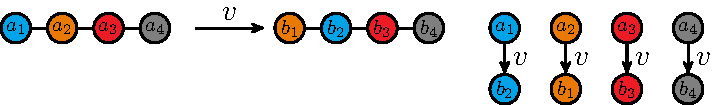
\includegraphics[]{case-1.pdf}
        \caption{}
        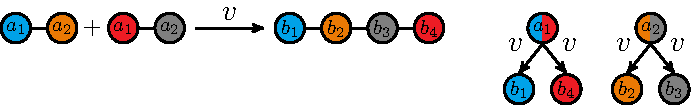
\includegraphics[]{case-2.pdf}
        \caption{}
        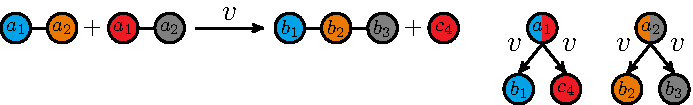
\includegraphics[]{case-3.pdf}
        \caption{}
        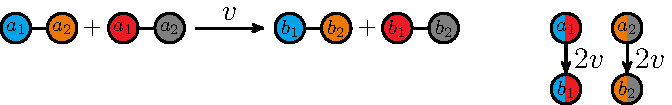
\includegraphics[]{case-4.pdf}
        \caption{}
        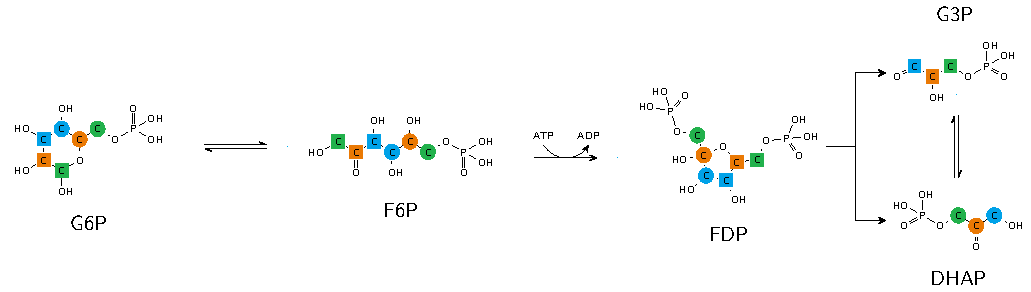
\includegraphics[width=12.0cm]{case-1-bio-example.pdf}
        \caption{}
        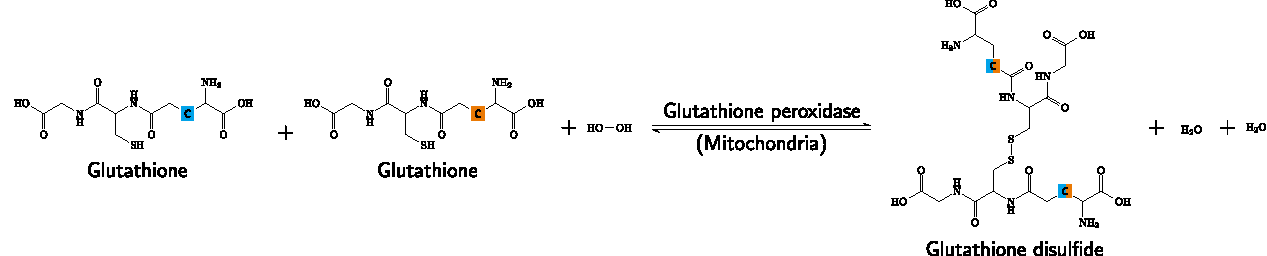
\includegraphics[width=12.0cm]{case-2-bio-example-inkscape.pdf}
        \caption{}
        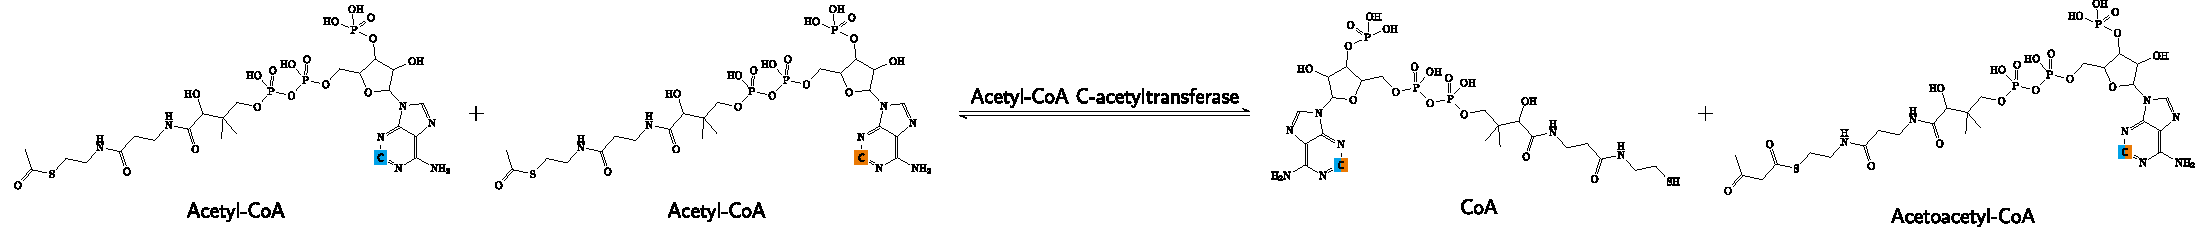
\includegraphics[width=12.0cm]{case-3-bio-example-inkscape.pdf}

    \end{subfigure}
\end{figure}

\end{document}
